% template.tex, dated April 5 2013
% This is a template file for Annual Reviews 1 column Journals
%
% Compilation using ar-1col.cls' - version 1.0, Aptara Inc.
% (c) 2013 AR
%
% Steps to compile: latex latex latex
%
% For tracking purposes => this is v1.0 - Apr. 2013

\documentclass[letterpaper]{ar-1col}
\usepackage{showyourwork}
\usepackage[letterpaper]{geometry}

\usepackage{natbib}
\usepackage{amsmath}
\usepackage{color}
\usepackage{hyperref}
\hypersetup{hidelinks}

\usepackage{graphbox}
\newcommand{\suz}[1]{\textcolor{magenta}{#1}}
\newcommand{\dan}[1]{\textcolor{green}{#1}}

\setcounter{secnumdepth}{4}
\usepackage{url}

% Metadata Information
\jname{Xxxx. Xxx. Xxx. Xxx.}
\jvol{AA}
\jyear{2022}
\doi{10.1146/((please add article doi))}

% autoref formatting
\def\sectionautorefname{Section}
\let\subsectionautorefname\sectionautorefname
\let\subsubsectionautorefname\sectionautorefname

% macros
\newcommand{\apjl}{Astrophysical Journal Letters}
\newcommand{\aj}{Astronomical Journal}
\newcommand{\apj}{Astrophysical Journal}
\newcommand{\apjs}{Astrophysical Journal Supplement}
\newcommand{\pasp}{Publications of the Astronomical Society of the Pacific}
\newcommand{\jgr}{Journal of Geophysical Research}
\newcommand{\aap}{Astronomy and Astrophysics}
\newcommand{\mnras}{Monthly Notices of the Royal Astronomical Society}
\newcommand{\actaa}{Acta Astronomica}
\newcommand{\nat}{Nature}
\newcommand{\prl}{Physical Review Letters}

% Symbols
\newcommand{\ydata}{\ensuremath{\boldsymbol{y}}}
\newcommand{\hyperparams}{\ensuremath{\boldsymbol{\phi}}}
\newcommand{\meanparams}{\ensuremath{\boldsymbol{\theta}}}
\newcommand{\dt}{\ensuremath{\tau}}
\newcommand{\amplitude}{\ensuremath{\alpha}}
\newcommand{\lengthscale}{\ensuremath{\lambda}}

\DeclareMathOperator*{\argmax}{arg\,max}

% Document starts
\begin{document}

% Page header
\markboth{Aigrain \& Foreman-Mackey}{GPR for Astronomy}

% Title
\title{Gaussian Process regression for astronomical time-series}

%Authors, affiliations address.
\author{Suzanne Aigrain,$^1$ and Daniel Foreman-Mackey$^2$
  \affil{$^1$Department of Physics, University of Oxford, Oxford, UK, OX1 3RH; email: suzanne.aigrain@physics.ox.ac.uk}
  \affil{$^2$Center for Computational Astrophysics, Flatiron Institute, New York, USA, NY 10010}}

%Abstract
\begin{abstract}
  Abstract text, approximately 150 words.
\end{abstract}

%Keywords, etc.
\begin{keywords}
  keywords, separated by comma, no full stop, lowercase
\end{keywords}
\maketitle

%Table of Contents
\tableofcontents

\section{INTRODUCTION}
\label{sec:intro}

\begin{armarginnote}[]
  \entry{GP}{Gaussian Process}
  \entry{GPR}{Gaussian Process Regression}
\end{armarginnote}

Gaussian Processes (GPs) are a powerful class of statistical models, which allow us to define a probability distribution over random functions. Rather than write down an explicit mathematical formula for the function from which some observations are generated, we model the covariance between pairs of samples from the process, using our physical domain knowledge and/or available data to guide our modelling.
While this may seem abstract, GPs have a wide range of applications from modelling of stochastic physical processes, to high dimensional interpolation and smoothing.
In particular, GP Regression (GPR) has become increasingly popular in the astronomical community over the last decade. Part of the reason for this uptake is the growing availability and importance of time-domain datasets in astronomy. These systematically contain non-trivial random or unknown signals, whether astrophysical or instrumental, that need to be modelled. In many cases, these are nuisance signals, which we need to marginalise over in order to detect or measure other signals robustly. Sometimes, we are interested in the stochastic behaviour itself, and want to infer its characteristics or predict its behaviour. GPR offers a compelling solution: statistically principled, naturally Bayesian, and extremely flexible, yet mathematically simple. To new users, however, the lack of an explicit functional form for the model can make GPR can seem a little arcane. Furthermore, the computational cost of the method, which scales cubically with the dataset size, can be an obstacle. These factors initially impeded its dissemination in the astronomical community, but have been largely overcome in recent years thanks to the availability of user-friendly, computationally optimised software packages.

\dan{Add some summary text here. ``In this review...''}

% In this review, we start with a broad and pedagogical introduction to GP methodology in theory and practice.
% We then work through many examples of how GPs have been used in the astronomical literature.
% Discuss

\suz{Should we mention we are using showyourwork?}

\subsection{Brief history}

An early use of GPR, was for spatial interpolation in geophysics \citep{kriging}, and GPR has since been adopted or re-invented in a wide range of other application domains. GPs were used in simulations in a wide range of astronomical sub-fields \citep[see e.g.][]{1980asfr.symp..159B,1988JGR....9311569C,1997ApJ...483L...1P}, but early mentions of GPs for modelling astronomical datasets \citep[see e.g.][]{1976MitAG..38..192D,1978A&A....70..777V,1991MGeo...16..313J} received limited attention.

Perhaps the earliest use of GPR in the refereed astronomical literature that will be familiar to a modern reader was published by \citet{prh92a} in the context of quasar variability, and for a long time this remained its main application domain in astronomy. GPR then gradually appeared in other areas, starting with photometric redshift estimation \citep{2006ApJ...647..102W}, then exoplanet transit observations \citep{2009ApJ...704...51C,2012MNRAS.419.2683G} and radial velocity planet searches \citep{2012MNRAS.419.3147A,2014MNRAS.443.2517H}. Nonetheless, GPR remained relatively niche and few astronomers had heard of it until a few years ago. To illustrate this point, we searched on the NASA Astrophysics Data System (ADS) for articles published in refereeed astronomy and astrophysics journals with the words ``Gaussian Process'' in full text of the article \autoref{fig:literature}.
After an increase in popularity throughout the 1990s, the use of GPs in astrophysics remained fairly constant around $\sim20$ publications per year until 2010.
Since 2010, the popularity of GPs has grown significantly, and in 2021, more than 500 refereed papers referencing GPs were published in the astrophysics literature.

A number of important factors have contributed to recent the democratisation of GPR across a wide range of scientific disciplines, including the publication of a dedicated textbook \citep{gpml}, as well as the availability of cheap computing power and user-friendly, open-source GPR software. In astronomy, specifically, an additional factor has been at play: the rise of time domain surveys. Correlated noise in time-domain observations is a direct and unavoidable consequence of causation, and hence ubiquitous. Adequately modelling this correlated noise is vital when searching for faint signals, for example from exoplanets. Astrophysical sources, from accretion disks on all scales to magnetically active stars or cloudy brown darfs, also display complex, intrinsically or apparently stochastic behaviour, for which adequate modelling strategies are required. GPR is a natural choice to tackle these challenges. Rather than attempting to cover all applications of GPs to all of astrophysics, which would not be feasible in the space available, we have therefore opted to focus on its application to time-domain datasets in astronomy.

\begin{figure}[ht]
  \centering
  \script{literature.ipynb}
  \includegraphics[width=0.5\linewidth]{figures/literature.pdf}
  \caption{The number of referred publications in the astronomy and astrophysics literature that include the text ``Gaussian process'' as indexed by the NASA Astrophysics Data System (ADS).}
  \label{fig:literature}
\end{figure}

\subsection{Motivating examples}
\label{sec:sim_examples}

By way of motivation, before delving any further into the methodology, we have produced two illustrative examples that highlight some typical use cases for GPR in astrophysics.
These examples are not meant to comprehensively summarize the space of use cases.
Similarly, the goal of this section is not to formally compare the performance of GPR to other methods with the same goals.
Instead, these examples are meant to identify some common, but qualitatively different applications.
In both examples, we use simulated datasets since it is useful to know the ``ground truth'' to validate performance.

The first example is a re-implementation of one of the earliest uses of GPR in time-domain astronomy \citep{prh92a}, using modern language and techniques.
In this example, we measure the time delay of a lensed quasar, using a GP as a flexible, non-parametric model for the latent (un-observed) variability of the unlensed quasar system.

The second example demonstrates the use of GPR to account for stellar variability in the light curve of a transiting exoplanet, when inferring its parameters.
In this case, the parameters of interest are the parameters of the mean model, and the GP is a nuisance model, and our goal is to propagate uncertainty introduced by the stellar variability to our constraints on the physical parameters of interest.

These examples---and all the examples throughout this review---are implemented using \textsf{tinygp} \dan{add tinygp Zenodo ref}, a \textsf{Python} library for GPR built on top of the \textsf{JAX} library for numerical computing \dan{add JAX ref}.
Here and throughout, the probabilistic models are implemented using the \textsf{NumPyro} library \dan{add NumPyro reference} and the Markov chain Monte Carlo (MCMC) inference is performed using the No U-Turn Sampling (NUTS) algorithm \citep{Hoffman:2014}.

\subsubsection{Example 1: The time delay of a gravitational lensed quasar}
\label{sec:quasar}

In this example, we re-visit the method developed by \citet{prh92a} to measure the time delay of the gravitationally lensed quasar 0957+561, one of the earliest applications of GPR for time domain astronomy.
The underlying model here is that the unobserved latent variability of the source is modelled using a GP, in this case we use a Mat\'ern-3/2 covariance function as discussed and defined in \autoref{sec:kernels}.
The images sample this time series at lagged times and with different mean magnitudes and variability amplitudes.

Under this assumed model, we simulate a pair of light curves with the same cadence and uncertainties as the dataset from \citet{1989A&A...215....1V} that was analyzed by \citet{prh92a}.
In this simulation, the parameters of the covariance model, the mean magnitudes, and the time delay are all set to known values, designed to produce qualitatively similar features to the dataset from \citet{1989A&A...215....1V}.
The simulated light curves are plotted in the left panel of \autoref{fig:quasar}.

Using these simulated data, we fit a GP model using MCMC, varying the time delay, the mean magnitude of each image, the variability amplitude of each image, and the timescale of the covariance.
The results of this inference are shown in \autoref{fig:quasar}.
In the left panel we show the simulated data with the median of posterior time delay applied to image A, and an arbitrary magnitude offset applied to image B for plotting purposes.
Over-plotted on these data are 12 posterior samples of the GP model predictions for the noise-free photometry for each image.
This figure captures how a GP can be used to flexibly capture a stochastically variable process under certain smoothness constraints, and how the uncertainties on the interpolated and extrapolated predictions increase away from the observed data.

The right panel of \autoref{fig:quasar} shows the posterior constraints for two of the key parameters of the model: the time delay, and the mean magnitude difference between images.
Since these are simulated data, we know the true values of these parameters, and these true values are over-plotted on \autoref{fig:quasar}b, demonstrating that our method reliably recovers the expected result.

\begin{figure}[ht]
  \centering
  \script{quasar.ipynb}
  \begin{minipage}[t]{0.5\linewidth}
    \includegraphics[width=\linewidth,vshift=1cm]{figures/quasar.pdf}
  \end{minipage} \hfill
  \begin{minipage}[t]{0.44\linewidth}
    \includegraphics[width=\linewidth]{figures/quasar_posteriors.pdf}
  \end{minipage}
  \caption{The results of fitting the simulated light curves of two images of a lensed quasar with a time delay between images.
  \emph{Left:} The simulated light curves for each image with an arbitrary magnitude offset applied to image B, and the median of posterior time delay applied to image A, bringing the light curves into a common frame.
  The data are plotted as points with error bars, and over-plotted on these data are posterior predictive samples of each images' predicted variability.
  \emph{Right:} The posterior constraints on the time delay and mean magnitude offset between the two images, obtained using Markov chain Monte Carlo (MCMC) to fit the simulated data shown in the left panel of this figure.
  The true values of these parameters that were used to simulate the data are over-plotted as blue lines.}
  \label{fig:quasar}
\end{figure}

\subsubsection{Example 2: Fitting an exoplanet transit with stellar variability}
\label{sec:transit}

In this second example, we demonstrate another common application of GPR in astrophysics, as a flexible model for nuisances and correlated noise where we want to correctly capture uncertainty introduced by this noise model into our constraints on the parameters of interest.
To this end, we simulate the light curve of a transiting exoplanet and aim to infer the physical parameters of the system, taking correlated noise into account.
The correlated noise in transit light curves is typically caused by the variability of the host star and by instrumental effects like focus or pointing changes.
It has been demonstrated that neglecting to account for these variations can cause significant errors when inferring the properties of the planet \citep{2006MNRAS.373..231P,2007A&A...472L..13G}.
This correlated noise can often be well-modeled by a GP, and the use of GPs for transit modeling has been a fruitful area of research in the astrophysics literature (see Section~\ref{sec:transit_fit} for a more detailed discussion).

For this example, the transit was simulated with known physical properties such as the planet-to-star radius ratio, the impact parameter, and quadratic limb darkening parameters \dan{cite Agol for light curve computation}.
We then add correlated and white noise by sampling from a GP model with a Mat\'ern-3/2 covariance function as defined in \autoref{sec:kernels}, with a known amplitude, timescale, and white noise amplitude.
These simulated data are shown in the left panel of \autoref{fig:transit}.

We then used the same framework to model the simulated dataset, first ignoring the correlated noise and then accounting for it explicitly.
For the transit model, we fit for the planet-to-star radius ratio $R_{\rm p}/R_\star$, the mid-transit time $T_0$, the out-of-transit flux $f_0$, and the limb darkening parameters $u_1,\,u_2$.
When also fitting for correlated noise, we also marginalise over the amplitude $\amplitude$ and timescale $\lengthscale$ of the GP model.
The posterior constraints on the time of transit and the planet-to-star ratio are shown in the right panel of \autoref{fig:transit}, with the true values of these parameters over-plotted as a black line.
When the correlated noise is neglected (plotted in orange in \autoref{fig:transit}), the inferred parameters are significantly inconsistent with the truth.
Taking the correlated noise into account (blue in \autoref{fig:transit}) increases the uncertainties on the inferred parameters, but also shifts the results to recover the true parameters.

\begin{figure}[ht]
  \centering
  \script{transit.ipynb}
  \begin{minipage}[t]{0.5\linewidth}
    \includegraphics[width=\linewidth,vshift=1cm]{figures/transit.pdf}
  \end{minipage} \hfill
  \begin{minipage}[t]{0.44\linewidth}
    \includegraphics[width=\linewidth]{figures/transit_posteriors.pdf}
  \end{minipage}
  \caption{The results of fitting the simulated light curve of a transiting exoplanet.
  \emph{Left:} The simulated dataset plotted as points with error bars.
  The inferred model when correlated noise is (blue) or isn't (orange) taken into account are over-plotted on the data.
  \emph{Right:} The posterior constraints on the time of transit $T_0$ and the planet-to-star radius ratio $R_\mathrm{p}/R_\star$.
  The colors in this figure match those in the left panel, and the true values of these parameters are indicated with black lines.
  The results when neglecting correlated noise (orange) are significantly inconsistent with the true value, but when the correlated noise is modeled using a GP (blue), the correct parameters are recovered, albeit with larger uncertainty.}
  \label{fig:transit}
\end{figure}


\subsection{Overview of this review}

The remainder of this review is structured as follows. Section~\ref{sec:basics} provides a brief, accessible introduction to the basic theory of GPR, and Section~\ref{sec:choices} discusses the key modelling choices one needs to make when using a GP to model data, with practical advice for how to make these choices. Section~\ref{sec:uses} gives an overview of applications of GPR to time-domain astronomical datasets to date. \suz{describe remaining sections}


% Heading 1
\section{BASICS OF GAUSSIAN PROCESS REGRESSION}
\label{sec:basics}

So far we have discussed how GPR has become widely used in astronomy and touched on some of their pros and cons, but we haven't explicitly defined what a GP is or explained how GPR works. This section gives a brief introduction to the theory of GPR, written in a way that we hope will be intelligible to most astronomers. For more details and practical exercises, we refer the reader to \citet{gpml} and \textcolor{red}{[Cite SA Saas Fee lecture notes if published]}.

\subsection{Formal definition}
\label{sec:def}

A GP is a type of \textit{stochastic process} based on the Gaussian probability distribution. A probability distribution describes a random variable with a finite number of dimensions. A stochastic process extends this concept to an infinite number of dimensions, allowing us to define a probability distribution over functions. Just what do we mean by ``extending to an infinite number of dimensions"? Well, this can be a little problematic mathematically, but we needn't worry about it, because in practice we only ever deal with finite samples from the stochastic process.

The formal definition of a GP is that the joint probability distribution over any finite sample $\mathbf{y} = (y_1, y_2, \ldots, y_n)^{\rm T}$ from the GP is a multi-variate Gaussian:
\begin{equation}
    p(\mathbf{y}) = \mathcal{N}(\mathbf{m}, \mathbf{K}),
\end{equation}
where $\mathbf{m}$ is the \emph{mean vector} and $\mathbf{K}$ the \emph{covariance matrix}.

The elements of the mean vector and covariance matrix are given by the \textit{mean function} $m$ and the \textit{covariance function} $k$, respectively:
\begin{equation}
    m_{i} = m(\boldsymbol{x}_i, \meanparams),
\end{equation}
\begin{equation}
    K_{ij} = k(\boldsymbol{x}_i,\boldsymbol{x}_j, \hyperparams).
\end{equation}
where $\boldsymbol{x}_i$ is the set of inputs (independent variables) corresponding to the $i^{\rm th}$ sample. For time-series data, the inputs usually include, but aren't necessarily restricted to, the time $t_i$. The covariance function, also known as the \emph{kernel}, is the fundamental ingredient of a GP model, and considerable care must be taken to select it adequately (or to test different possibilities). Sometimes the mean function is assumed to be constant, or even zero, everywhere; this is often done in the wider GPR literature to keep derivations uncluttered. However, for many astrophysical applications where a GP is used to model a nuisance signal, the mean function contains the signal of interest and is important.

The parameters $\meanparams$ and $\hyperparams$ of the mean and covariance function are known as the \textit{hyper-parameters} of the GP. Strictly speaking, the \textit{parameters} of the GP are the (infinitely many) unknown functions that share the specified mean vector and covariance matrix and could have given rise to the observations. However, these parameters are always marginalised over: we never explicitly deal with the individual functions, except when drawing samples for illustrative purposes (as we did in Figures~\ref{fig:quasar} and \ref{fig:transit}). GPs are therefore a type of \textit{Hierarchichal Bayesian hierarchical Model} (HBM). 

Although is is possible to construct and use stochastic process models based on other distributions, GPs are by far the most popular, for two main reasons. The first is Central Limit theorem: it implies that the assumption of Gaussianity is often at least approximately correct. The second is that Gaussian distributions obey simple mathematical identities for marginalisation and conditioning, that inference with GPs (the process of marginalising over the individual functions) to be performed \textit{analytically}, with very simple linear algebra. It is this analytic marginalisation property that sets GPR apart from other forms of HBM. \suz{ask Dan to check these last two paragraphs.}

\subsection{From least-squares to GPR}
\label{sec:from_lsq}

The formal definition above does not necessarily provide an intuitive understanding of how GPs work. Most readers of this review will, however, be more familiar with least-squares regression. In this section we will show that GPR can be thought of as a generalisation of least-squares regression, allowing for correlated noise (or signals) in the data. Conversely, least-squares regression, as traditionally presented, is a special case of GPR, where the covariance matrix is assumed to be purely diagonal, and the variances associated with each observation are known \textit{a priori}.

\subsubsection{Revisiting least squares}\label{sec:lsq}

Consider $N$ observations of a variable $\mathbf{y} = \{ y_i\}_{i=1, \ldots, N}$, taken at times $\mathbf{t} = \{ t_i\}$, with associated measurement uncertainties $\boldsymbol{\sigma}=\{\sigma_i\}$. We wish to compare these to a model function $m(t,\meanparams)$ controlled by parameters $\meanparams=\{\meanparams_j\}_{j=1,\ldots,M}$. In most astrophysical applications, we are interested in estimating some or all of those parameters. In least-squares regression, we minimize the quantity
\begin{equation}
  \chi^2 \equiv\sum_{i=1}^N (y_i-m_i)^2/\sigma^2_i,
\end{equation}
where $m_i \equiv m(t_i,\meanparams)$, with respect to $\meanparams$. Where does this come from?

Let us assume that the observations are given by
\begin{equation}
  y_i=m(t_i,\meanparams)+\epsilon_i,
\end{equation}
where $\epsilon_i$ is the measurement error, or noise, on the $i^{\rm th}$ observation. Furthermore, let us assume that $\epsilon_i$ is drawn from a Gaussian distribution with mean $0$ and variance $\sigma_i^2$:
\begin{equation}
  p(\epsilon_i)=\mathcal{N}(0,\sigma_i^2) \equiv \frac{1}{\sqrt{2\pi} \sigma_i} \exp\left(-\frac{\epsilon_i^2}{2\sigma_i^2} \right),
\end{equation}
then the \emph{likelihood} for the $i^{\rm th}$ observation is simply
\begin{equation}
  \mathcal{L}_i\equiv p(y_i|\meanparams)=\mathcal{N}(m_i,\sigma_i^2) =\frac{1}{\sqrt{2\pi} \sigma_i} \exp\left[-\frac{(y_i-m_i)^2}{2\sigma_i^2} \right].
\end{equation}
Furthermore, we also assume that the noise is uncorrelated, or white, meaning that the $\epsilon_i$'s are drawn independently from each other from their respective distributions. Then, the likelihood for the whole dataset $\mathbf{y}$ is merely the product of the likelihoods for the individual observations:
\begin{equation}
  \mathcal{L} \equiv p(\mathbf{y}|\meanparams) = \prod_{i=1}^N \mathcal{L}_i = \prod_{i=1}^N \left\{ \frac{1}{\sqrt{2\pi} \sigma_i}
  \exp\left[-\frac{(y_i-m_i)^2}{2\sigma_i^2} \right] \right\},
\end{equation}
where $\mathbf{m}=\{m_i\}_{i=1,\ldots,N}$. From this one can readily see that $\ln \mathcal{L} = \mathrm{constant} - 0.5 \chi^2$, where the constant depends only on the $\sigma$'s. Thus, if the $\sigma$'s are known, maximizing $\mathcal{L}$ is equivalent to minimizing $\chi^2$. In other words, least-squares regression yields the Maximum Likelihood Estimate (MLE) of the parameters under the assumption of white, Gaussian noise with known variance.

\subsubsection{Link to Gaussian Process Regression}\label{sec:gp-lsq-link}
\dan{I think we should explicitly re-write this as $\mathcal{L}(\meanparams,\,\hyperparams)$ and indicate that $K$ and $m$ depend on these parameters. We should really highlight that this is a drop-in replacement for the likelihood defined in the previous section.} \suz{Is this ok?}
Let us now re-write the likelihood in matrix form:
\begin{equation}
\label{eq:gp_like}
  \mathcal{L}(\meanparams,\hyperparams) = 
  \frac{1}{\sqrt{|2\,\pi\,\mathbf{K}|}} \exp \left(-(\mathbf{y}-\mathbf{m})^{\mathrm{T}} \mathbf{K}^{-1}
  (\mathbf{y}-\mathbf{m}) \right),
\end{equation}
where, as before, the mean vector $\mathbf{m}$ has elements $m_i=m(t_i,\meanparams)$ and $\mathbf{K}$ is a purely diagonal ($N$, $N$) matrix with elements $K_{ij} = \delta_{ij} \sigma_i^2$ ($\delta_{ij}$ being the discrete Kronecker delta function). This is, of course, the \emph{covariance matrix} of the model.

Now, instead of assuming that the covariance matrix takes this very specific form, let us allow a more flexible covariance model:
\begin{equation}
  K_{ij} = k(t_i,t_j,\hyperparams) + \delta_{ij} \sigma_i^2,
\end{equation}
where $k$ is a \emph{covariance function} or \emph{kernel}, controlled by parameters $\hyperparams$. The result is a GP, and its likelihood is still given by Equation~(\ref{eq:gp_like}). Depending on the choice of kernel and parameters, the covariance matrix can now have non-zero off-diagonal elements, allowing us to explicitly model correlated noise or stochastic signals in the data.
Note that the likelihood depends not only on the argument of the exponential, but also on the determinant of the covariance matrix, which therefore needs to be evaluated explicitly. This term acts as a built-in Occam's razor, automatically penalising more complex models.

The kernel $k$ encodes our beliefs about the stochastic, or random, element of the model, in just the same way as the mean function $m$ encodes our beliefs about the deterministic component of the model. For example, in many circumstances, we would expect that two observations taken close together in time should be more strongly correlated than observations taken further apart, and we would use a decreasing function of the time interval $\dt=|t_i-t_j|$ to represent that. One of the most widely used covariance functions is the squared exponential
\begin{equation}
  k(\dt;\,\hyperparams) = \amplitude^2\,\exp\left(-\frac{\dt^2}{2\,\lengthscale^2}\right)
\end{equation}
This gives rise to smooth random functions with variance $\amplitude$ and characteristic length-scale $\lambda$. We present other commonly used kernels and discuss how to select one in Section~\ref{sec:kernels}.

\subsection{Inference with a GP}\label{sec:gp-inf}

% \begin{figure}[ht]
%   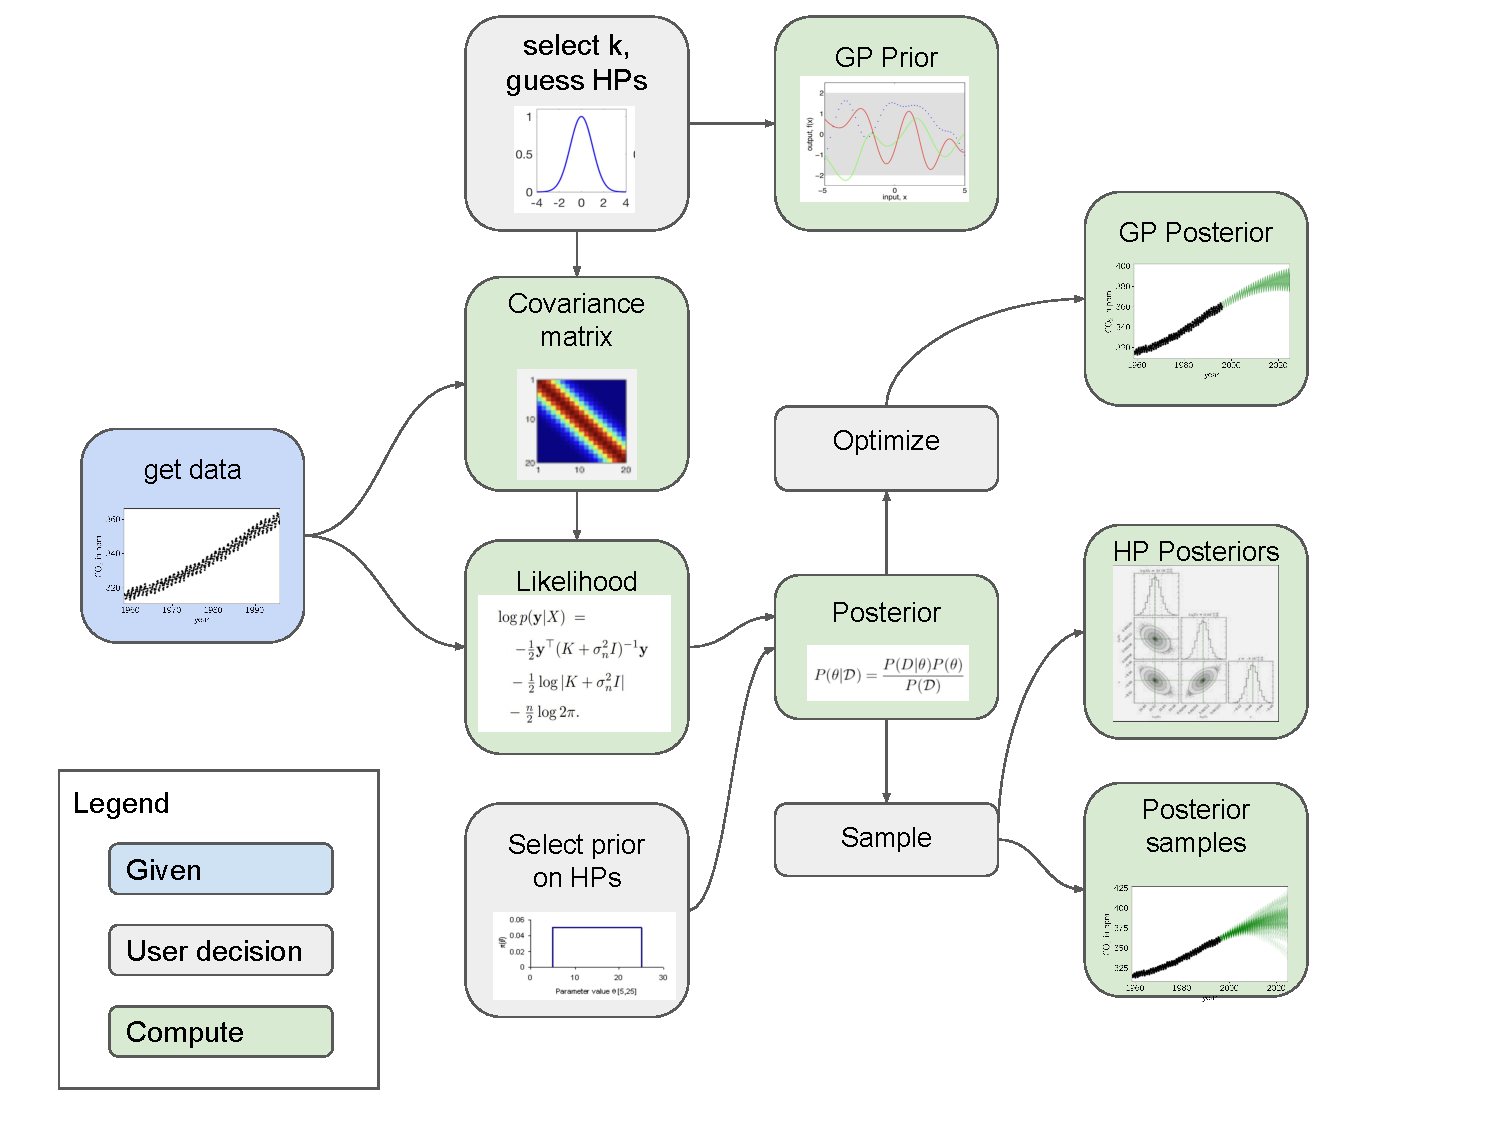
\includegraphics[width=\linewidth]{GPR_workflow.pdf}
%   \caption{Schematic of the workflow for Bayesian inference with a GP. The process starts with getting some data (blue box), and making some choices about how we are going to model it (grey boxes, these choices are discussed in Section~\ref{sec:choices}). The mathematical framework presented in this section can then be used (green boxes) to evaluate the likelihood and posterior distribution over the HPs which can be optimized or sampled. We can also condition the GP on the data to predict observations at locations where we do not yet have observations. \suz{Figure will be updated with nicer version.}}
%   \label{fig:GPRworkflow}
% \end{figure}

Now that we know how to evaluate the likelihood (Equation~\ref{eq:gp_like}), we are ready to perform \textit{inference}, that is to use observations to update our prior beliefs about the system we are observing. The overall Bayesian inference workflow for GPR regression is illustrated schematically in Figure~\ref{fig:GPRworkflow}. For example, we can optimize the likelihood with respect to the hyper-parameters $\hyperparams$ and $\meanparams$. In the machine learning literature, where GPs are commonly used, this is called \emph{training} the GP. In doing so, we are learning the properties of the correlated signal from the data.

Given adequate priors, we can also evaluate the \emph{posterior} distribution:
\begin{equation}
  p(\meanparams,\hyperparams|\mathbf{y})=\frac{p(\mathbf{y}|\meanparams,\hyperparams)p(\meanparams,\hyperparams)}{p(\mathbf{y})},
\end{equation}
where $p(\mathbf{y})=\int p(\mathbf{y}|\meanparams,\hyperparams)p(\meanparams,\hyperparams) \mathrm{d}\meanparams \mathrm{d}\hyperparams$.
Usually, the posterior cannot be evaluated analytically, so we resort to sampling methods such as Markov Chain Monte Carlo (MCMC) or nested sampling.

In many astrophysical applications of GPs, we wish to take into account correlated noise, but we are not interested in the noise \emph{per se}, only on the impact it has on the parameters of the mean function, $\meanparams$. We thus \emph{marginalize} (integrate over) the \emph{nuisance parameters} $\hyperparams$.


\subsection{Making predictions}
\label{sec:pred}

\begin{figure}[ht]
  \centering
  \script{GPR_PGM.ipynb}
  \includegraphics[width=\linewidth]{figures/GPR_PGM.pdf}
  \caption{Probabilistic Graphical Model (PGM) got GP regression (adapted from Figure 2.3 of \citealt{RW07}). The top layer shows the (known) inputs $\{t\}$}
  \label{fig:GPR_PGM}
\end{figure}

An important use case for GPR is as a statistically principled interpolation method. We wish to ``learn'' an unknown function that gave rise to some data, in order to make predictions for some new set of inputs. Importantly, a GP model provides not a point estimate but a full probability distribution for the function at any desired location(s) in the input domain. This allows for robust uncertainty propagation (though there are some important caveats we will touch upon), and can also motivate strategies for active sampling (deciding when or where to make new observations).

\subsubsection{The predictive equations}

Given some existing observations $\mathbf{y}$, taken at times $\mathbf{t}$, how do we make predictions at some new set of times $\mathbf{t}_\star$? We are after $p(\mathbf{y}_\star|\mathbf{y})$, the \textbf{conditional} probability distribution for $\mathbf{y}_\star$ given $\mathbf{y}$. In GPR this is also known as the \emph{predictive distribution}, because it is often used to extrapolate a time-series dataset forwards. The `magic' of GPR is that the predictive distribution is also Gaussian, and its mean and covariance are given by simple analytic relations:
\begin{equation}
  \label{eq:pred}
  \mathbf{f}_\star = \mathbf{m}_\star + \mathbf{K}_\star^{\mathrm{T}} \, \mathbf{K}^{-1} \, (\mathbf{y} - \mathbf{m}) ~\mathrm{~~~and~~~}
  \mathbf{C}_\star =   \mathbf{K}_{\star\star} - \mathbf{K}_\star^{\mathrm{T}} \, \mathbf{K}^{-1} \, \mathbf{K}_\star,
\end{equation}
where we have introduced the notation $\mathbf{m}_\star \equiv m(\mathbf{t}_\star,\meanparams)$, $\mathbf{K}_\star \equiv k(\mathbf{t},\mathbf{t}_\star, \hyperparams)$ and
$\mathbf{K}_{\star\star} \equiv k(\mathbf{t}_\star,\mathbf{t}_\star,\hyperparams)$. Note that, as real observations are always noisy, $\mathbf{K}$ generally includes a white noise term ($\delta_{ij} \sigma^2_i$), but $\mathbf{K}_\star$ does not. Depending on whether one wishes the predictive variance (the diagonal elements of $\mathbf{C}_\star$)  to account for measurement uncertainties or not, one can include the white noise term in $\mathbf{K}_{\star\star}$ or leave it out.

\subsubsection{Properties of the  predictive distribution}
A closer look at Equations~(\ref{eq:pred}) reveals some important properties.
First, a GP is a \textit{linear predictor}. The predictive mean for a specific time $t_\star$ can be written as a linear combination of the observations:
$f_\star = \mathbf{w}^{\mathrm{T}} \, \mathbf{y}$, where $\mathbf{w} = \mathbf{K}^{-1} \, \mathbf{k}_\star$ and $\mathbf{k}_\star=k(\mathbf{t},t_\star,\hyperparams)$. It can also be written as
a linear combination of covariance functions centred on the training points:
$f_\star = \mathbf{\alpha}^\mathrm{T} \,  \mathbf{k}_\star$ where $\mathbf{\alpha} = \mathbf{K}^{-1} \, \mathbf{y}$.
These linearity properties are very important to understand the behaviour of GPs. They shed light on the relationship between GPR and standard linear models with very large numbers of free parameters \citep[see e.g.][for a more detailed discussion]{2021PASP..133i3001H},
and lead to a number of powerful extensions that are beyond  scope of this review.

Second, the predictive covariance is independent of the data. $\mathbf{C}_\star$ depends only on the \emph{locations} $\mathbf{t}$ of the observations, not on their values $\mathbf{y}$. This has important consequences for observation planning: if we know the covariance function $k$ and its parameters, we can decide when to observations to optimise our predictions at a given (set of) time(s). However, in practice we rarely know the hyper-parameters \textit{a priori}, and the predictive posterior distribution marginalised over the hyper-parameters \textit{does} depend on the observations.

Finally, as $\mathbf{K}$ is positive semi-definite, so is $\mathbf{K}^{-1}$. Therefore, $\mathbf{k}_\star^{\mathrm{T}} \, \mathbf{K}^{-1} \, \mathbf{k}_\star \ge 0,$ and $\mathrm{Var}(\mathbf{f}_\star) \leq k(t_\star,t_\star)$. This is as we would expect: obtaining more data should only ever improve the accuracy of our predictions.

\subsubsection{Cautionary notes}

It is important to note that the behaviour of $\mathbf{f}_\star$ is \emph{not} the same as that of individual samples from the predictive distribution. Typically,  $\mathbf{f}_\star$ tends to be smoother than individual samples. This should be borne in mind when displaying GPR results or using them in subsequent analysis.

It is also important to note that the predictive variance accounts for the imperfect ability of the specific model under consideration to explain the data, but not for the choice of model (i.e. the choice of mean and kernel functions and their parameters). We discuss how to choose a kernel function and fit for its parameters in the next section.

\section{GAUSSIAN PROCESS MODELING DECISIONS}
\label{sec:choices}

% Assigned: DFM

% \paragraph{Kernels} Selecting a kernel function is how the user builds physical domain knowledge into the Gaussian process model. In this section, we will both try to dispel some common misconceptions about how to choose covariance functions and their parameters, and provide some practical guidelines for how to make these modelling choices in practice, highlighting specific examples from the astronomical literature. Estimated length: 5-10 pages

% Question: will this also be the section where the most commonly used kernel functions in astrophysics are introduced or will that be part of section1? This will affect the relative length of the two sections, but overall I'd expect it to be 15-20 pages for both sections

% \paragraph{Tuning} This section will cover the process of "training" a Gaussian process model, i.e. tuning the parameters of the covariance function and, if included, the mean function. Compared to standard texts from other fields, this topic will be covered in more depth because parameter inference (as opposed to interpolation or prediction) is one of the most common applications of Gaussian processes in astronomy. Once again we will aim to dispel some misconceptions and provide practical advice. This will also be where we illustrate how a Gaussian process model can be embedded in a Bayesian inference framework using posterior sampling, and point out the importance of marginalising over nuisance parameters. Estimated length: 5-10 pages


In the previous section, we presented an overview of GP methods, and the key mathematical details. In this section, we will dive deeper into some of the practical decisions that arise when using GPs.
The two core elements of a GP model are the mean function $m(t;\,\meanparams)$, and the ``kernel'' or ``covariance'' function $k(t_i,\,t_j;\,\hyperparams)$.
Unlike how they are typically presented in the machine learning literature, GP models in astrophysics will often---but not always---include non-trivial mean functions.
For example, in the example from \autoref{sec:transit}, the mean function $m(t;\,\meanparams)$ is a physical transit model that is a function of the orbital parameters of the system, and includes a realistic limb-darkening model \citep{2002ApJ...580L.171M}.
However, in this review we won't discuss the mean function in detail, focusing instead primarily on the kernel function, since that is unique to GP modeling.
All this being said, in our experience, new users of GP models will often focus and worry more than necessary about the choice of kernel function for their problem.
As with any probabilistic modeling problem, there are several well-defined workflows for motivating, selecting, and validating your choice of kernel.
In this section we walk through this process in detail.

\subsection{Gaussian Process Covariance Functions}
\label{sec:kernels}

\dan{Say something about to handle higher dimensional inputs and distance metrics.}

\begin{textbox}[htb]
  \section{Kernel function}
  The ``kernel'' or ``covariance'' function, typeset here as $k(t_i,\,t_j;\,\hyperparams)$ is a parametric description of the covariance between two data points $t_i$ and $t_j$. The parameter $\hyperparams$ indicates that these functions are typically parameterized by a set of parameters, typically referred to as ``hyper-parameters''.

  \vspace{1.5em}

  \section{Hyper-parameters}
  In a GP model, the kernel function is typically parameterized by a set of parameters that we will label as $\hyperparams$ and refer to as ``hyper-parameters''.
  Formally, the ``parameters'' of a GP are the (unknown) ``true'' values of the process at the observed times, but the magic of Gaussians means that these parameters can be marginalised over in closed form, leaving the hyper-parameters as the parameters of interest.
\end{textbox}

The kernel function can be any positive semi-definite scalar function, but some will be more useful than others.
% A commonly (over-)used kernel function is the ``exponential-squared'' or ``radial basis function'' kernel
% \begin{equation}
%   k(t_i,\,t_j;\,\hyperparams) = \sigma^2\,\exp\left[-\frac{(t_i - t_j)^2}{2\,\tau^2}\right]
% \end{equation}
% where the ``hyperparameters'' $\hyperparams$ are $\sigma$ and $\tau$.
% In this case, the hyperparameters specify the typical amplitude $\sigma$ and timescale $\tau$ of the variance of the process.
% SOMEFIGURE shows how changing these parameters affect our GP model.
% There exist many other commonly used kernel functions, some of which are listed in SOMETABLE.
% This table is far from comprehensive, and importantly, the sum or product of two valid kernel functions is itself also a valid kernel, so it is possible (and common) to build extremely flexible and expressive kernel functions specific to your use case.
Given this large decision space, you may be wondering how to choose the right kernel for your specific problem.
If you're very lucky, you may be able to motivate your model using physics.
This can be approached from two directions.
On one hand, some commonly used kernel function have a specific physical interpretation---for example, the solution to a stochastic ordinary differential equation---that can be used to motivate their use.
On the other hand, if your physical model is specified by its \emph{power spectrum}, this can recast as a GP model with a specific kernel function. \suz{Say something about the number of times a function is differentiable? That can be a useful consideration. But perhaps already mentioned later.}

Even if you don't have a formal physics-based justification for your model, you may be able to identify the key scales of your problem and design a kernel function that captures these features.
The usual approach to this problem is to take sums and products of commonly used kernel functions to select a set of  models that have the needed covariance structure, and then combine or select between these choices.
For example, if there is only expected to only be a single non-periodic timescale in the problem of interest, you could list all the two-parameter non-periodic kernels and use a numerical model selection technique as described below.

\subsubsection{Standard kernels \& sums or products thereof}

Some popular kernels are listed in \autoref{tab:kernels}, and some other choices are discussed in Chapter 4 of \citet{gpml}.
In any practical application, these kernel functions are not used on their own.
Instead, more expressive models are designed by combining these models.
In particular, any valid kernel functions can be added or multiplied to generate new valid functions.
For example, the squared exponential kernel function is generally defined as
\begin{equation}
  k(\dt;\,\hyperparams) = \amplitude^2\,\exp\left(-\frac{\dt^2}{2\,\lengthscale^2}\right)
\end{equation}
with $\hyperparams = \{\amplitude,\,\lengthscale\}$, which, in our notation, is actually the product of a constant kernel and a squared exponential kernel, as defined in \autoref{tab:kernels}.
Another example that is commonly used in the astrophysics literature \citep{2012MNRAS.419.3147A,2014MNRAS.443.2517H} is the following ``quasi-periodic'' kernel
\begin{equation}
  k(\dt;\,\hyperparams) = \amplitude^2\,\exp\left(-\frac{\dt^2}{2\,{\lengthscale_1}^2} -\gamma\,\sin^2\left[\frac{\pi\,\dt}{\lengthscale_2}\right] \right)
\end{equation}
with $\hyperparams = \{\amplitude,\,\lengthscale_1,\,\lengthscale_2,\,\gamma\}$, which has a period of $\lengthscale_2$, and a decoherence timescale of $\lengthscale_1$.

When selecting a kernel function, it can be useful to generate samples from this implied prior distribution over functions to get a qualitative sense of the properties of the kernel.
In practice, this is done by choosing a grid of times $\boldsymbol{t} = \{t_i\}$, evaluating the elements of the covariance matrix
\begin{equation}
  K_{i,j} = k(t_i,\,t_j;\,\hyperparams) \quad,
\end{equation}
and then generating a multivariate Gaussian sample with this covariance.
As an example, \autoref{fig:samples} shows several prior samples for three different kernel functions from \autoref{tab:kernels}, with a range of length scales $\lengthscale$ and amplitudes $\amplitude$.
In this figure, we can see some qualitative differences between the kernels---namely that the kernels become ``smoother'' from left to right---and we can see how the range of allowed functions change with the hyper-parameters.

\begin{table}[ht]
  \caption{Some kernel functions commonly used in the astrophysics literature \dan{add the rational quadratic kernel}}
  \label{tab:kernels}
  \begin{center}
    \begin{tabular}{@{}l|l@{}}
      \hline
      Name                           &  Representation$^{\rm a}$                                    \\
      \hline
      Constant kernel                & $\amplitude^2$                                                     \\
      Squared Exponential$^{\rm b}$  & $e^{-(\dt/\lengthscale)^2/2}$                                              \\
      Exponential$^{\rm c}$          & $e^{-\dt/\lengthscale}$                                                  \\
      Mat\'ern-3/2                   & $\left(1 + \sqrt{3}\dt/\lengthscale\right)e^{-\sqrt{3}\dt/\lengthscale}$             \\
      Mat\'ern-5/2                   & $\left(1 + \sqrt{5}\dt/\lengthscale +5(\dt/\lengthscale)^2/3\right)e^{-\sqrt{5}\dt/\lengthscale}$  \\
      Cosine                         & $\cos 2\pi\dt/\lengthscale$                                                  \\
      Exponential Sine Squared       & $\exp\left(-\gamma\sin^2\pi\dt/\lengthscale\right)$                      \\
      Stochastic Harmonic Oscillator$^{\rm d}$ & $\cos\left(\sqrt{1-\beta^2}\frac{\dt}{\lengthscale}\right) + \frac{\beta}{\sqrt{1-\beta^2}}\sin\left(\sqrt{1-\beta^2}\frac{\dt}{\lengthscale}\right)$                          \\
      \hline
    \end{tabular}
  \end{center}
  \begin{tabnote}
    $^{\rm a}$in each case, $\dt$ is defined as $\dt = \left|t_i - t_j\right|$, and Greek letters indicate hyper-parameters;
    $^{\rm b}$``radial basis function'';
    $^{\rm c}$``Ornstein-Uhlenbeck'', ``damped random walk'' or ``Mat\'ern-1/2'';
    $^{\rm d}$\citet{celerite}.
  \end{tabnote}
\end{table}

\begin{figure}[ht]
  \centering
  \script{samples.ipynb}
  \begin{minipage}[t]{0.3\linewidth}
    \includegraphics[width=\linewidth]{figures/samples1.pdf}
  \end{minipage} \hfill
  \begin{minipage}[t]{0.3\linewidth}
    \includegraphics[width=\linewidth]{figures/samples2.pdf}
  \end{minipage} \hfill
  \begin{minipage}[t]{0.3\linewidth}
    \includegraphics[width=\linewidth]{figures/samples3.pdf}
  \end{minipage}
  \caption{Prior samples for three different classes of kernel functions: (a) exponential, (b) Mat\'ern-3/2, and (c) exponential squared.
  In each sub-figure, the length scale $\lambda$ of the kernel increases from left to right, and the amplitude $\alpha$ increases from top to bottom.
  One thing to notice in this figure is that these kernel functions differ in their smoothness properties.
  Specifically, the exponential kernel is not mean-square differentiable, while the exponential squared kernel is infinitely differentiable.
  This can be seen qualitatively in this figure.}
  \label{fig:samples}
\end{figure}

\subsubsection{Operations on kernel functions}

As discussed above, more flexible kernel models are often constructed using products and sums of the standard kernels listed in \autoref{tab:kernels}.
Besides, addition and multiplication, other operations can be used to impose structure on the standard kernels.
For example, linear operations like scalar multiplication, differentiation, or integration can all be used to develop new kernel functions.

For example, there are good arguments \dan{CITE} to expect that the radial velocity time series of a spotted rotating star is related to the photometric time series via its time derivative.
More formally, assume we have two time series---one with observations of some function $f(t)$ and another with observations of $\dot{f}(t)$, where the dot indicates the derivative with respect to time---and the function $f(t)$ is modeled as a GP with some covariance function $k(t_i,t_j;\hyperparams)$.the covariance between $f(t)$ and $\dot{f}(t)$ is
\begin{equation}
  \mathrm{Cov}\left[f(t_i),\dot{f}(t_j)\right] = \left.\frac{\mathrm{d}k(t_i,t;\hyperparams)}{\mathrm{d}t}\right|_{t=t_j}
\end{equation}
and the covariance $\dot{f}(t)$ and itself is
\begin{equation}
  \mathrm{Cov}\left[f(t_i),\dot{f}(t_j)\right] = \left.\frac{\mathrm{d}^2k(t,t^\prime;\hyperparams)}{\mathrm{d}t\,\mathrm{d}t^\prime}\right|_{t=t_i,t^\prime=t_j} \quad.
\end{equation}
This means that we can compute the GP model for observations of both sets of observations and their covariances.
\autoref{fig:kernel-ops} shows some examples of this. \dan{more and citations}

Similarly, integration or convolution also have similar properties.
For example, real time series observations are made with finite exposure time $\Delta$, and therefore, if the underlying stochastic process $f(t)$ is modeled as a GP with covariance $k(t_i,t_j;\hyperparams)$, the observations are actually of
\begin{equation}
  f_\mathrm{int}(t) = \int_{t-\Delta/2}^{t+\Delta/2} f(t^\prime)\,\mathrm{d}t^\prime \quad,
\end{equation}
which has a covariance of
\begin{equation}
  k_\mathrm{int}(t_i,t_j;\hyperparams) = \int_{t_i-\Delta/2}^{t_i+\Delta/2}\int_{t_j^\prime-\Delta/2}^{t_j+\Delta/2} k(t,t^\prime;\hyperparams)\,\mathrm{d}t\,\mathrm{d}t^\prime \quad,
\end{equation}
which can be evaluated in closed form for some standard kernel functions.
Another context where integrated GPs has been used for astrophysics (albeit not for time series), is as a model of the Galactic dust distribution \dan{CITE}.

\begin{figure}[ht]
  \centering
  \script{kernel-ops.ipynb}
  \includegraphics[width=0.7\linewidth]{figures/kernel-ops1.pdf}
  \includegraphics[width=0.7\linewidth]{figures/kernel-ops2.pdf}
  \caption{Derivative kernels.}
  \label{fig:kernel-ops}
\end{figure}


\subsubsection{Multivariate GPs}

Since this review is focused on GPs for \emph{time domain} astronomy, we primarily consider univariate GPs with just \emph{time} as the input coordinate.
However, we would be remiss to neglect discussing multivariate GPs altogether.
Most of our discussion so far applies to multivariate datasets without any change, but there are some subtleties that are worth mentioning here.

When working with univariate GPs, it is relatively straightforward and unambiguous to compute the ``distance'' between two points $t_i$, and $t_j$: $\rho(t_i,t_j) = \dt = \left|t_i - t_j\right|$.
For multivariate inputs $\boldsymbol{x}$, more care must be taken to define a sensible distance metric $\rho(\boldsymbol{x}_i,\boldsymbol{x_j})$.
Common choices include the $d$-th norm $\rho_d(\boldsymbol{x}_i,\boldsymbol{x_j}) = \left|\left|\boldsymbol{x}_i - \boldsymbol{x}_j\right|\right|_d$ for $d=1$ or $d=2$, but other metrics---for example, the Haversine distance when the elements of $\boldsymbol{x}$ are coordinates on a sphere---might be better motivated for a particular use case.

A common class of multivariate GP model for time domain astronomy are datasets with multiple parallel covariant time series.
For example, multi-band time series produced by surveys like PanSTARRS or LSST, or radial velocity time series with parallel activity indicators.
One useful way to specify these datasets are to define the inputs as $\boldsymbol{x_i} \equiv (t_i,\ell_i)$ where $t_i$ the time of the $i$-th observation and $\ell_i$ is a ``label'' for which time series the $i$-th observation is drawn from.

Abs vs other norms, non-standard geometry (GPs on the sphere), parallel time series.

\subsubsection{Physically motivated kernels}

Cosmology, asteroseismology, etc.

\suz{Mention kernels with break points to detect sudden changes, as described in review by \citet{2012RSPTA.37110550R} for example?}

\subsection{Hyperparameter Inference}

A key component of all the covariance functions discussed above is that they are all \emph{parameterized} by a set of hyper-parameters.
In most cases, you won't have \emph{a priori} knowledge for how the values of these hyper-parameters should be set.
Instead, their values will need to be numerically tuned or incorporated into a larger inference scheme.

In the astrophysics literature, the most common approach for taking this uncertainty into account---and the method that we advocate for here---is to treat the hyper-parameters directly as parameters of the model.
In other words, instead of just fitting for the parameters of the mean model $\meanparams$, we can simultaneously fit for both $\meanparams$ and the hyper-parameters $\hyperparams$.
In \autoref{sec:gp-lsq-link}, we defined the likelihood for a GP model and, in \autoref{sec:gp-inf}, we sketched the procedure used for Bayesian inference with such a model.
The likelihood function defined in \autoref{eq:gp_like} is a function of both $\meanparams$ and $\hyperparams$, and we can use that function as an objective for a non-linear optimization routine to find the maximum likelihood parameter values, or in a Markov chain Monte Carlo (MCMC) procedure to marginalise over the hyper-parameters, and propagate their uncertainty to constraints on the parameters of the mean model.

An important point here is that, since many data analysis procedures in astrophysics include a step like the ones listed above, the use of a GP likelihood doesn't significantly change the processing.
In fact, we like to say that the GP likelihood can be used as a drop-in replacement for anywhere you're currently using a ``chi-squared'' objective.
There are some practical reasons why things aren't necessarily this simple (for example, computational cost, as described below), but the sentiment stands.

In this review, we won't go into too many details about the inference algorithms, but throughout the text, we will regularly use the \textsf{BFGS} gradient-based, non-linear optimization routine \citep{Nocedal:1999, scipy} to find the maximum likelihood parameter values
\begin{equation}
  \meanparams_\star,\hyperparams_\star = \argmax_{\meanparams,\hyperparams} \,\mathcal{L}(\meanparams,\hyperparams) = \argmax_{\meanparams,\hyperparams} \,\log p(\ydata\,|\,\meanparams,\hyperparams) \quad.
\end{equation}
Another common inference technique used in astrophysics---and in this review!---is the use of Markov chain Monte Carlo (MCMC) to generate posterior samples
\begin{equation}
  \meanparams,\hyperparams \sim p(\meanparams,\hyperparams\,|\,\ydata)
\end{equation}
that can be used to marginalise over some subset of the parameters, and estimate the uncertainty on the parameter values.
All the examples in this review are implemented using the \textsf{NumPyro} probabilistic inference library, and all the MCMC examples use the gradient-based No U-Turn Sampler (NUTS) algorithm \citep{Hoffman:2014}.

\autoref{sec:quasar} and \autoref{sec:transit}, and specifically \autoref{fig:quasar} and \autoref{fig:transit}, show the results of worked examples of an MCMC-based GPR workflow, without and with (respectively) a non-trival mean function.


\subsection{Model assessment, validation, and selection}

Given the wide array of possible kernel functions described in \autoref{sec:kernels}, it can be important to assess the performance of your model and the relevant choices.
This includes both assessing the choice to use a GP in the first place, and the specific choice of kernel function.
It's important to note that there's nothing fundamentally different about GPs in the context when compared to other models for data, so that means that many methods that you may already use for model selection and validation in other contexts will also apply when using GPs.
That being said, within the astrophysics literature formal probabilistic model checking has had limited use, and GPs do come with some specific technical complications, therefore we will discuss some examples of model validation and selection techniques that have been used for GPs.

\dan{Say something here about assessing Gaussianity.}

When it comes to selecting between different possible kernel functions, the approach that you take may depend on your specific research goals.
For example, in many cases, including the transiting exoplanet example in \autoref{sec:transit}, the main parameters of physical interest may be the parameters of the mean model, and the GP is simply an effective model for stochastic nuisances.
In this case, it may be sufficient to demonstrate that the inferred results are not significantly inconsistent for different choices of kernel function.

Other common use cases, like the time delay example in \autoref{sec:quasar}, primarily require good predictive performance for the GP model.
In these cases, methods like cross-validation of posterior predictive assessment \dan{add link to Gelman paper here} can be used to evaluate different choices of kernel function.

To demonstrate these approaches, \autoref{fig:assessment} shows the results of performing a model comparison between three different kernel functions applied to a simulated dataset.
The simulated data were generated from a GP model with a squared exponential kernel with known parameters, and we aim to compare the performance of three kernels: (1) the squared exponential kernel, (2) the Mat\'ern-3/2 kernel, and (3) the rational quadratic kernel.
The simulated dataset is shown in the left panel of \autoref{fig:assessment}.

First, using the full dataset, we compute the Bayesian evidence integral for each of these model choices using a nested sampling algorithm implemented in the \textsf{jaxns} package \dan{add citation}.
The Bayesian evidence integral is defined as:
\begin{equation}
  Z(H) \equiv p(\ydata\,|\,H) = \int p(\meanparams,\hyperparams\,|\,H)\,p(\ydata\,|\,\meanparams,\hyperparams,H)\,\mathrm{d}\meanparams\,\mathrm{d}\hyperparams
\end{equation}
where $H$ indicates the modeling choices, in this case the choice of kernel function.
For better or worse\footnote{A discussion of the relative merits of different model selection algorithms is beyond the scope of this review. \suz{Sure but can we link to a more in-depth discussion of the topic for interested readers?}}, the Bayesian evidence is frequently used in the astrophysics literature as an ingredient in model selection procedures.
Nested sampling is an algorithm for numerically estimating this integral, and we apply it to produce estimates of $Z$ for each choice of kernel $H$, and plot these results in the middle panel of \autoref{fig:assessment}.
In this figure, it is clear that the squared exponential and rational quadratic kernels are indistinguishable under this metric, while the Mat\'ern-3/2 kernel is somewhat disfavoured. 

Another popular method for model selection that is less commonly used in the astrophysics literature is cross validation.
Cross validation is designed to assess the predictive performance of the model, and it proceeds by holding out some data, fitting the rest of the data, and then computing the likelihood of the held out data conditioned on the fit results.
These steps can then be repeated for different held out samples.
For a GP model, the likelihood of the held out data can be computed using the predictive distribution discussed in \autoref{sec:pred}.
In particular, the likelihood is the following multivariate Gaussian
\begin{equation}\label{eq:held-out-like}
  p(\ydata_\star\,|\,\ydata,\meanparams, \hyperparams) = \mathcal{N}(\boldsymbol{f}_\star,\boldsymbol{C}_\star)
\end{equation}
where $\boldsymbol{f}_\star$ and $\boldsymbol{C}_\star$ are defined in \autoref{eq:pred}, noting (importantly!) that the (squared) observational uncertainties on the held out data should be included on the diagonal of $\boldsymbol{C}_\star$.

In this example, we use MCMC to fit the data shown as black dots in the left panel of \autoref{fig:assessment}, holding out the data points indicated by blue crosses.
At each step in the MCMC, we evaluate the likelihood in \autoref{eq:held-out-like} for the held out data conditioned on the training data and the model parameters.
In the rightmost panel of \autoref{fig:assessment}, we plot the posterior distribution of the held out log probability to show that, like with the evidence integral, the squared exponential and rational quadratic kernels are indistinguishable, while the Mat\'ern-3/2 kernel is disfavoured. 
\suz{Maybe mention leave-p-out CV as a more realistic CV strategy for real applications?}

\begin{figure}[ht]
  \centering
  \script{assessment.ipynb}
  \includegraphics[width=\linewidth]{figures/assessment.pdf}
  \caption{Model assessment.}
  \label{fig:assessment}
\end{figure}


% Heading 3
\section{GAUSSIAN PROCESSES IN TIME-DOMAIN ASTRONOMY}
\label{sec:uses}

In this section we discuss a range of applications of GPR to time-domain datasets in the astronomical literature. The present-day popularity of GPs in astronomy precludes any attempt at an exhaustive review. Instead, we have selected examples which showcase the power and flexibility of the method. The order in which these applications are discussed is partly based on chronological considerations, but we have also attempted to present the simpler applications first.d


\subsection{Stars and exoplanets}
\label{sec:stars_planets}

It is no coincidence that the recent uptake of GPR in astronomy coincides with the meteoritic rise of exoplanet studies. Almost all exoplanet detections and related discoveries are made indirectly, and involve detecting small and/or short-lived signals in time-domain datasets: transits in light curves, Keplerian signals in Radial Velocity (RV) or astrometry time-series. These are invariably affected by, and often buried in, correlated noise or nuisance signals, making GPR a natural choice.

%The search for exoplanets has also motivated the development of large-scale time-domain photometric and spectroscopic surveys, a by-product of which is the study of a wide range of stellar astrophysics phenomena, where GPR has also found fresh applications that will be discussed later in this Section. Historically, the first applications of GPR to exoplanet datasets were for transit modelling.

\subsubsection{Transit searches}
\label{sec:transit_det}

Following the discovery of the first transiting exoplanet \citep{2000ApJ...529L..41H,2000ApJ...529L..45C}, numerous ground-based photometric monitoring surveys were set up (or re-purposed) to search for planetary transits. Early estimates of their yield \citep[see e.g.][]{2003ASPC..294..361H} ran into the hundreds of planets per year, but these soon turned out to be highly optimistic. While surveys such as the Optical Gravititational Lensing Experiment (OGLE) did indeed discover numerous transit-like events
%\citep{2002AcA....52....1U,2002AcA....52..317U,2003AcA....53..133U,2004AcA....54..313U}
\citep[see e.g.][]{2002AcA....52....1U}, only a handful were ultimately confirmed as bona-fide transiting planets, and the process took years. %\citep{2003Natur.421..507K,2003ApJ...597.1076K,2004ApJ...609L..37K,2005ApJ...624..372K,2004A&A...421L..13B,2004A&A...426L..15P}.
The vast majority of early transit candidates were later diagnosed as diluted or grazing stellar eclipses based on radial velocity follow-up.
%\citep{2005A&A...431.1105B,2005A&A...438.1123P}.
Intriguingly, a small fraction turned out to be spurious detections, despite having relatively high signal-to-noise ratio (SNR). Indeed, \citet{2006MNRAS.373..231P} noted that all the confirmed OGLE planets had very high SNRs, and went on to show that the SNRs for all candidates had been over-estimated due to the presence of correlated, or red, noise in the light curves. They proposed an empirical method to evaluate the red noise on transit time-scales from the individual light curves (analogous to the method proposed by \citealt{prh92a} to evaluate the correlation matrix of a quasar light curve), and then a prescription for adjusting the detection threshold accordingly. In effect, they were searching for a way to model the covariance of the data. This is precisely what GPR allows, but the methodology was not known in the exoplanet community at the time.

GP models have been used on occasion to \textit{detrend} light curves from transit surveys prior to running transit searches, i.e.\ to remove variability on timescales significantly longer than a transit \citet[see e.g.][]{2016ApJS..226....7C}, and are used frequently after detection to model the out-of-transit baseline alongside the transit signal itself (see next sub-section). In principle, a GP could also be used to model out-of-transit variations (intrinsic or instrumental) alongside transits as part of a detection pipeline. Doing this simultaneously rather than sequentially allows more flexible models to be used for the out-of-transit variations, and avoids the risk of corrupting the transit signal by using an excessively aggressive filter at the detection stage, as demonstrated by \citet{2015ApJ...806..215F} for \textit{K2} data. In that case, the primary source of out-of-transit variability is instrumental systematics (see next section), which are to some degree common to all light curves in a given observing run. \citet{2015ApJ...806..215F} model these systematics as a linear combination of the first 150 principal components of the ensemble of light curves, alongside a simple box-shaped transit model, varying the latter's period, phase and duration.

In other space-based transit surveys such as \textit{CoRoT}, \emph{Kepler} and \emph{TESS}, the systematics are less prominent, so the dominant source of out-of-transit variations is intrinsic stellar variability, which occurs mainly on timescales longer than transits, and can therefore be filtered out quite effectively without removing the transits. However, in some cases, for example for rapidly rotating and magnetically active stars, the separation between transits and stellar signal becomes less clean, significantly reducing the performance irrespective of sequential detrending approaches (irrespective of the algorithm used, \citealt{wotan}).
In such cases, a simultaneous modelling approach could improve detection performance significantly. Since the nuisance signal is specific to each star, it cannot be modeled using other light curves, but a GP is a credible alternative. Such an approach could also offer a small but significant enhancement in the sensitivity future missions such as \textit{PLATO} to transits of habitable planets around Sun-like stars (which are very shallow and relatively long). The main issue would be computational cost: transit surveys monitor $10^4$--$10^5$ stars at a time, with $10^3$--$10^5$ observations per run, and the transit search must be run over a fine grid of periods and phases. Doing this with standard GPR methods would be impractical. However, now fast and scalable GP solvers are available, this becomes a more feasible proposition.

\subsubsection{Transit and eclipse modelling}
\label{sec:transit_fit}

In practice, GPR has been much more widely applied to transit modelling than to detection \textit{per se}. The detailed depth, timing, duration and shape of a transit depends on the planet-to-star radius ratio $R_{\rm p}/R_\star$, the system scale $a/R_\star$ (where $a$ is the orbital semi-major axis), the impact parameter $b$, the orbital period $P$ and the time of transit centre, $T_0$ as well as the limb-darkening profile of the star. High-precision observations of one or more transits of a given planet can be used to infer these parameters, which has a wide range of scientific applications. The most obvious is to estimate the planet size (and hence, given a mass estimate, its bulk density and composition [ref]). The system scale is directly related to the stellar density [ref seager-mallen03], which can be used for sanity checks to ensure the transits are indeed of planetary origin [ref tingley]. Small departures from strictly periodic timing, known as Transit Timing Variations (TTVs), probe dynamical interactions between multiple planets in a given system, and can be used measure the planets' masses and eccentricities and to reveal the presence of additional, non-transiting planets [ref]. Wavelength-dependent measurements of the transit depth probe the effect of the planet's atmosphere on the star light that filters through it, and hence allow us to access the atmospheric composition. The depth of any secondary eclipse (when the planet passes behind the star) depends on the planet-to-star flux ratio, and can therefore be used to measure an emission or reflection spectrum, while its timing yields strong constraints on the orbital eccentricity. All of this requires precise and accurate measurements of the transit parameters, for which any correlated noise must be accounted for explicitly, as we demonstrated using a simulated example in Section~\ref{sec:transit}.


To address this, \citet{2009ApJ...704...51C} proposed a wavelet-based method to model correlated noise in transit light curves, which can be seen as a special case of GPR with a covariance function belonging to the exponential family, but the formulation using wavelets. Rather than modelling the covariance in the time domain, the Power Spectral Density (PSD) of the noise is assumed to be of the form $P(f) \propto f^{-\gamma}$.
Noting that the wavelet transform of such a process gives rise to a nearly diagonal covariance matrix, \citet{2009ApJ...704...51C}  derived an expression for the likelihood that can be computed in $\mathcal{O}(N)$ operations. This method has been used widely since its publication to model transit observations from space missions which stare continuously at a given field, such as \textit{Kepler} or \textit{TESS}. However, the use of a wavelet transform requires regular time sampling, which precludes its application to datasets with irregular sampling or significant data gaps, for example from space telescopes in low-Earth orbit such as Hubble and Spitzer.
\begin{armarginnote}
  \entry{Colours of noise}{White, pink and red noise correspond to $\gamma=0$, $1$ and $2$, respectively.}
\end{armarginnote}


This limitation is significant, as Hubble and Spitzer have been the workhorse instruments for transit and eclipse spectroscopy for over a decade. This involves measuring minute changes in the depth of the primary transit or secondary eclipse as a function of wavelength, either using successive photometric observations through different filters or using a spectrograph (see \citealt {2018haex.bookE.100K} for a review). The signal of interest is the wavelength dependence of the transit depth, or the depth of the eclipse, which are of order $10^{-4}$ and $10^{-3}$ respectively, in  the most favourable cases. Even when observed from space, these signals are typically dwarfed by instrumental systematics. The pointing jitter and thermal relaxation of the telescope as it orbits the Earth causes the target star to move on the detector, typically by a fraction of a pixel. As the sensitivity of the detector varies from pixel to pixel (the ``flat-field'') and between the centre and edges of each pixel, this motion causes spurious variations in the recorded flux from the target. Although we expect the measured flux to depend on ``housekeeping" variables such as the satellite orbital phase, telescope attitude, the centroid of the image or the locus and angle of the spectrum of the detector, or the temperatures of various parts of the instrument, a physically motivated model for the form of this dependence is generally lacking. \textit{Ad hoc} parametric (e.g.\ polynomial) models are problematic, as the choice of model inputs and functional form is arbitrary, yet can drastically alter the resulting exoplanet spectrum \citep{2011MNRAS.411.2199G}.

To address this, \citet{2012MNRAS.419.2683G} proposed a GPR framework to model the systematics in space-based transit observations. The aforementioned housekeeping variables are treated as multi-dimensional inputs to a squared exponential GP whose mean is the transit signal, allowing one to marginalise over broad families of systematic models without assuming a specific functional form for them, all the while propagating the resulting uncertainties on the physical parameter of interest, namely the (wavelength-dependent) planet-to-star radius ratio. The kernel used has a different length scale for each input dimension, but a single, shared output scale (or amplitude), known as an Automatic Relevance Determination (ARD) kernel:
\begin{equation}
    k_{\rm ARD}(\mathbf{x}_i, \mathbf{x}_j) = A \exp \left( - \sum_{m=1}^M \frac{|\mathbf{x}_i-\mathbf{x}_j|_m^2}{\lambda_m} \right),
\end{equation}
where $M$ is the number of input dimensions. Combined with ``shrinkage'' hyper-priors favouring long $\lambda$'s, this allows one to try including a wide range of housekeeping data into the fit; in principle only those which are genuinely relevant will have an effect on the result.
GP-based systematics models of this kind were later extended to eclipse spectroscopy, where the parameter of interest is the planet-to-star flux ratio, which controls the eclipse depth. Among other successes, this approach has enabled the first measurement of the wavelength-dependent albedo of a hot Jupiter \citep{2013ApJ...772L..16E}, helped resolve early controversies surrounding the treatment of systematics in Spitzer observations \citep{2015MNRAS.451..680E} and
led to the first unambiguous detection of a thermal inversion in an exoplanet emission spectrum \citep{2017Natur.548...58E}. Using simulated data, \citet{2014MNRAS.445.3401G} showed that GPs outperform parametric models when the true form of the systematics is unknown, but also that the most robust results overall are obtained by marginalising over families of both parametric and GP models.

Despite these theoretical advantages and practical successes, the use of GPR to analyse low-resolution transit and eclipse spectra remains confined to a relatively small subset of the corresponding community. Parametric models (in some cases marginalising over families thereof, [ref wakeford]) remain the most widely-used approach for Hubble space telescope observations, and Pixel-Level-Decorrelation (PLD) for Spitzer observations [ref Deming]. Possible explanations for this include computational cost, as well as the fact that these other methods are perceived as easier to implement and interpret. As the recently-launched JWST begins to deliver much higher signal-to-noise observations, multiple analyses of which by different groups are actively encouraged, it will be interesting to see how this topic evolves in the next few years.

One general shortcoming of current GP-based systematics models with multi-dimensional inputs is that the uncertainties on the input variables are ignored. This could in principle be remedied by treating the housekeeping variables as noisy observations of latent GP variables, and modelling them alongside the observed fluxes, but we are not aware of published attempts to do this in practice to date. \begin{armarginnote}
  \entry{Latent variable}{A random variable which is never actually observed.}
\end{armarginnote}
In spectroscopic observations, whether using GPs or parametric models, it has become standard practice to model the ``white" light curve first (obtained by integrating the spectrum over the full wavelength range at each time-step). ``Coloured'' light curves, extracted in individual wavelength bins, are then divided by the best-fit systematics model derived from the white light curve, before being modelled further. To our knowledge, no attempt has been made to model the wavelength dependence of the systematics directly.

On the other hand, GPR has become quite widely used for modelling correlated noise in single-band transit observations. One striking example is the case of transiting planet candidates discovered by \textit{Kepler} around giant stars. By comparing the stellar densities derived from transit modelling to those expected from independent estimates, \citet{2014ApJ...788..148S} argued that many of these candidates, including the confirmed planet Kepler-91, might be false positives. However, red giant light curves contain stochastic variability on timescales of hours due to granulation. In the case of Kepler-91, \citet{2015ApJ...800...46B} showed that the apparent density discrepancy disappears when this granulation signal is modelled using a GP.

\subsubsection{Systematics removal in the presence of stellar variability}
GP-based models have also been used to correct instrumental systematics in data from the \textit{K2} space mission, which used the \textit{Kepler} satellite to perform an Ecliptic plane survey after the failure of two of its reaction wheels. During the \textit{K2} observations, the satellite underwent significant roll-angle variations, causing the stars to move on the detector by more than a pixel over a timescale of hours. The satellite thrusters were fired every $\sim 6$\,h to return the spacecraft to its nominal attitude, but the resulting drift caused significant changes in the measured stellar fluxes, due to the detector inter- and intra-pixel variations, and to changes in the contamination of the photometric aperture by neighbouring targets as well as in aperture losses. These can be modelled effectively using a GP with a squared exponential covariance function depending on the roll angle \citep{2015MNRAS.447.2880A, 2016ApJS..226....7C} or the star's 2-D position on the detector \citet{2016MNRAS.459.2408A}. In these approaches, a second, time-dependent term is added to the GP covariance function to represent the target star's intrinsic variability. This not only improves the fit but allows the position-dependent systematics to be evaluated separately and thus removed while preserving intrinsic variability. The use of a time-depedent GP term improves the photometric performance over other widely-used methods for correcting \textit{K2} systematics \citep[e.g.][]{2014PASP..126..948V} when the stellar variability is significant and/or occurs on timescale similar to the roll angle variations. Ultimately, the best overall photometric precision for \textit{K2} was achieved by combining PLD to model the position-dependent systematics with a time-dependent GP to model intrinsic variability \citep{everest1,everest2}.

\begin{textbox}[ht]
\section{Composite GPs}
A composite (additive or multiplicative) GP is a powerful way to separate different components of a time-series dataset, whether these components depend on different input variables (as in the instrumental systematics examples discussed in this section) or not. To evaluate the predictive distribution for a particular component of a composite GP, one simply evaluates $\mathbf{K}_\star$ and $\mathbf{K}_{\star\star}$ in Equations~(\ref{eq:pred}) using that component only, while using the full covariance for $\mathbf{K}$.
\end{textbox}

\subsubsection{Quasi-periodic GP models for stellar light curves}

The light curves of Sun-like stars (broadly construed) display low-amplitude quasi-periodic variations which are caused by the rotational modulation and evolution of magnetically active regions on their surfaces. These produce quasi-periodic variations in both photometry and radial velocity observations, and GPs have in recent years become one of the most popular ways of modelling them. One reason for this is that a simple quasi-periodic covariance function  \suz{[refer to relevant section or introduce here]}, which reproduce the light curves of rotating stars with evolving active regions remarkably well.

%\suz{Some of this paragraph may be superseded by text in Section 3.} In particular, the following quasi-periodic (QP) kernel has proved especially popular to model stellar activity signals:
%\begin{equation}
%    k_{\rm QP} = A \exp\left[ - \Gamma \sin(\pi \tau / P) - \tau^2 / \lambda \right],
%\end{equation}
%where $A$ is the overall variance, $P$ is the period and $\Gamma$ controls the harmonic complexity of the periodic term, while $\lambda$ controls the evolution timescale. This is only one of many possible options: a valid quasi-periodic kernel can be constructed by multiplying together any valid periodic covariance function with any other valid covariance function that gives rise to a decaying envelope, and a valid periodic covariance function by replacing the argument(s) of an aperiodic one by a periodic function thereof. In this particular example, the periodic term $\exp[-\Gamma\sin^2(\pi t/P)]$ is obtained by considering a squared exponential in 2-D space $(u,v)$ and setting $u=\cos\tau$ and $v=\sin\tau$ [REF Mackay].

GP models were first applied to variations by \citet{2012MNRAS.419.3147A}, to test a new method to simulate Radial Velocity (RV) variations based space-based photometry on solar data. The context of this work was the large numbers of candidate transiting exoplanets being discovered at the time by the \textit{CoRoT} and \textit{Kepler} space missions. Detecting the planets signals in RV was needed to confirm the planetary nature of the candidates by measuring their masses, but was being hampered by the apparent RV variations caused by active regions. Using simple geometric considerations, \citet{2012MNRAS.419.3147A} derived a simple (approximate) relationship between the flux perturbation caused by active regions, $F$, and their RV signature, which depends on both $F$ and its time-derivative $F'$. They tested this data-driven ``$FF'$ method'' on simulated photometric and RV observations of the Sun-as-a-star produced using resolved magnetograms, using a GP as a principled smoothing tool to evaluate $F$ and $F'$ from the photometry, and comparing the results to the simulated RVs. \citet{2012MNRAS.419.3147A}  tested a number of covariance functions, both aperiodic and Quasi-Periodic (QP), and found the former to be preferred in the solar case. This is not entirely surprising, as the typical lifetimes of active regions on the Sun are not much longer than its rotation period [ref]. More active and/or more rapidly rotating stars display variability that is coherent over multiple rotation periods, making QP GPs the model of choice. For example, \citet{2014MNRAS.443.2517H} used a QP kernel when applying the aforementioned $FF'$ method to the active planet-host star CoRoT-7.

Today, using GPs to model light curves containing stellar variability is standard practice. The kernel most frequently used for this purpose is the aforementioned QP kernel, whose simplicity and flexibility make it a popular choice. \citep{2018MNRAS.474.2094A} implemented a Bayesian inference framework based on this kernel to measure accurate rotation periods from \textit{Kepler} light curves. The very complex dependence of the likelihood surface on the parameters, particularly the period, makes this challenging, and careful tuning of the posterior sampling strategy is required.

Although the QP kernel provides a phenomenological rather that physically motivated description of the variability, some of its parameters lend themselves to a physical interpretation in terms of the star's rotation period and the evolution timescale of active regions. \citep{2022MNRAS.tmp.2007N} tested this using simulated light and RV curves based on physical star-spot models and confirm that, for moderately well-sampled datasets, the period of the GP does indeed provide a precise and accurate measure of the stellar rotation period. The same is true, albeit to a lesser extent, for the evolution timescale: the correlation between simulated and recovered values is more scattered, and breaks down when the datasets spans less than the simulated evolution timescale.

On the other hand, the QP kernel (or any covariance function of time only) does not give access to the physical properties of the spots, such as their size, latitude or contrast. The problem of inferring these properties from light curves is fundamentally ill-posed \citep{2021AJ....162..123L}, making direct inference of individual spot properties or brightness maps highly degenerate (whatever the methodology used). However, \citet{2021AJ....162..124L} derive a closed-form expression for a GP that describes the light curve of a rotating, evolving stellar surface conditioned on a given distribution of starspot sizes, contrasts, and latitudes. This can be used in a hierarchical Bayesian framework to infer the distribution in question from ensembles of light curves.

Most studies focusing on the photometric signatures of stellar activity ignore variations on short timescales, either working with binned data or using a ``jitter term'' to absorb them. This keeps the model simple and, when binning, speeds up computing time. However, when the time-sampling and precision of the observations allow it (e.g.\ for data from \textit{CHEOPS} or \textit{PLATO}), composite GP models with different terms to describe activity, granulation and stellar oscillations can be useful. For example, \citet{2020A&A...634A..75B} analysed light curves of stars observed at high cadence and high precision in the \textit{CoRoT} asteroseismology field. They showed that the parameters of planetary transits injected into these light curves were recovered more accurately when using a composite GP to model the stellar variability than one with a single term. They also tested a white noise only model, which provided less precise precise estimates than either GP models, albeit generally consistent with both.

\subsubsection{Stellar activity in Radial Velocities}
Given the remarkable instrumental precision actived by modern RV spectrographs, stellar activity is nowadays the key factor limiting the sensitivity of RV surveys low-amplitude and/or long-period planet signals. The effect of active regions on RV observations is two-fold. First, as dark spots rotate on the stellar surface, they distort the profile of spectral lines, removing a small contribution first from the red wing of each spectral line, then from the line core, and then from the blue wing. The second effect is more subtle: in the absence of active regions, spectral lines of Sun-like stars display a net blue-shift due to granulation: the emission from the hot, up-welling material in the granules, which is blue-shifted, dominates over that from the cooler material falling back down in the inter-granular lanes). In a facula, i.e.\ a region of enhanced magnetic flux density compared to the ``clean'' photosphere, convection is suppressed, leading to a localised reduction in this ``convective blue-shift''. Faculae have very small photometric contrast but can cover a much larger area than dark spots, so their RV signature can dominate over that of spots, specially for moderately slow rotators like the Sun with modest magnetic fields \citep{2010A&A...512A..39M}.

\begin{figure}[ht]
  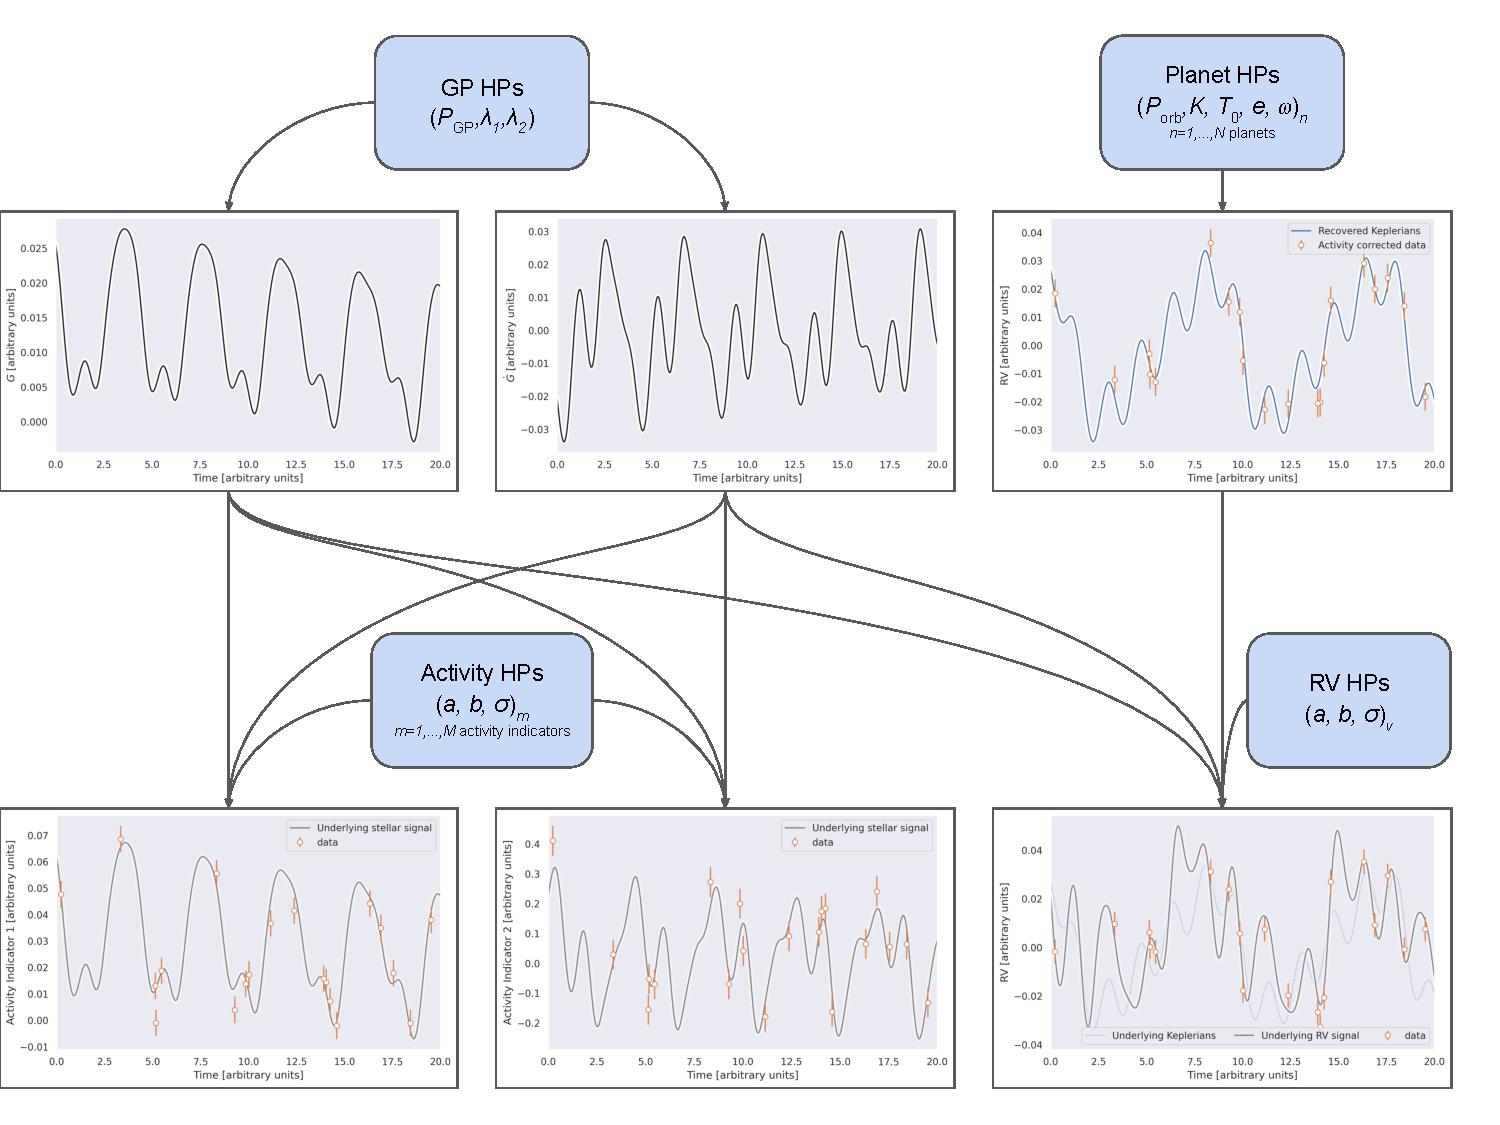
\includegraphics[width=3in]{static/RV_framework.pdf}
  \caption{Schematic of the GP framework of \citet{2015MNRAS.452.2269R} for modelling activity signals in RV data \suz{Figure will be updated with nicer version.}}
  \label{fig:RV_framework}
\end{figure}

Overall, active regions produce quasi-periodic RV variations which are frequently modelled with the same kind of QP GPs as for light curves. However, unlike transits, planetary signatures in RV occur on timescales similar to activity signals, meaning that the risk of overfitting is significant. This partly mitigated for RV follow-up of transiting planets by strong priors on the stellar rotation period and on the period and phase of the planetary orbit, but it is a severe problem for ``blind'' RV searches. The issue is compounded by the fact that RV observations are invariably ground-based, and strong pressure on telescope time means that the time-sampling of these observations is not always good enough to constrain the GP parameters well.

As previously alluded to, \citet{2012MNRAS.419.3147A} showed that an approximate relationship should exist between the photometric and RV signatures of active regions. Specifically, if $F(t)$ is the photometric signature and $F'(t)$ its time-derivative, the RV variations are expected to scale as $A F(t) F'(t) + B F^2(t)$, where the first term corresponds to spots and the second to faculae (assuming that the two are generally co-located, although the latter covers a larger area), and $A$ and $B$ are tunable free parameters. In its original form, however, this method was of limited applicability, as it requires the RV observations to be quasi-simultaneous with high-precision, tightly sampled light curves, which the case only exceptionally (see e.g.\ \citealt{2014MNRAS.445.3401G}).

On the other hand, RV extraction pipelines routinely provide additional indicators measuring the characteristic width and asymmetry of the spectral lines, which are also affected by active regions, as well as spectral activity indicators which trace chromospheric emission in the cores of strong lines. \citet{2015MNRAS.452.2269R} developed a GP framework, schematically illustrated in Figure~\ref{fig:multiGPRV}, to model these activity indicators alongside the RVs, and to disentangle them from planetary signals. Each observed time-series is modelled as a linear combination of some latent variable $G(t)$, its time derivative $G'(t)$, white noise, and (in the case of the RVs only) one or more Keplerian signals. $G(t)$ does not have a direct physical interpretation; it loosely corresponds to $F^2$ in the $FF'$ framework of \citet{2012MNRAS.419.3147A}, so that $G'(t) \propto F(t) F'(t)$, but it is modelled as a (typically quasi-periodic) GP, which makes it possible to write down expressions for the covariance between any pair of observations from the any of the time-series included in the analysis. This results in a global covariance matrix of dimensions $(NM,NM)$, where $N$ is the number of observations and $M$ the number of activity indicators included in the analysis. This framework has proved particularly successful for RV confirmation of transiting planets around young stars \citep{2019MNRAS.490..698B,2022MNRAS.512.3060Z}, enabling the detection of planetary signals almost 50 times smaller than the activity signals.  Open-source implementations of this framework have been published recently \citep{2022MNRAS.509..866B,2022A&A...659A.182D}, and extensions thereof are likely to play a significant role in the analysis of next regeneration RV surveys targeting Earth analogues, which need to achieve even better contrast between activity and planetary signals.

\subsubsection{Granulation and asteroseismology}


\suz{Possible addition: modelling high-dispersion spectra with GPs}

\subsection{AGN variability (DFM)}

\suz{This section is assigned to DFM but as I started writing something about it for the introduction then decided to move it here I have left it in -- feel free to use this as a starting point or ignore it entirely!.}

The Active Galactic Nuclei (AGN) at the centre of many distant galaxies produce stochastic variability in their optical and radio emission, on timescales ranging from hours to years.

\subsubsection{Lensed quasar time-delays}

As discussed in Section~\ref{sec:intro}, this is --to the best of our knowledge-- the first area in which GPR makes an appearance in the refereed astronomical literature.

\suz{Refer to the first simulated example in \autoref{sec:quasar} here. Some of the text below may need to move to that Section.}

When the quasar is lensed by an intervening galaxy or galaxy cluster, multiple images can be formed, whose brightness can be monitored individually. Measurements of the time-delays between the resulting light curves can be used to constrain the Hubble constant, $H_0$ \citep{doi:10.1146/annurev.aa.30.090192.001523}. Early measurements of these time-delays in the decade following the discovery of the first multiply imaged quasar, the ``double quasar'' 0957$+$561, were hampered by the lack of a generative model for the light curves. Heuristic methods based on interpolation and cross-correlation were developed, but uncertainties were difficult to derive and results obtained with different instruments and different bandpasses weren't always consistent. \citet{prh92a} derived a simple $\chi^2$ metric under the assumption that the observed light curves are shifted, noisy versions of a single sample a Gaussian process with known covariance. Having proposed an empirical procedure to estimate the covariance function from the data, they then optimize the $\chi^2$ with respect to the time-delay between images, and apply standard methods used to derive an uncertainty. While their method relied on an adhoc method to estimate the covariance matrix, and did not propagate the corresponding errors into the final result, it did resolve the prior discrepancy between the estimates of the time-delay from optical and radio dataets \citet{prh92b}. Even then, the requirement to invert the covariance matrix was a barrier to the wider application of this method. This was addressed a few years later by \citet{pr95}, who introduced introduced a fast algorithm, to invert the covariance matrix for exponential kernels. Updated versions of this algorithm now form the basis for fast GP solvers discussed in Section~\ref{sec:fast}.

\subsubsection{Reverberation mapping}

\subsubsection{Quasar power spectrum estimation}

\subsection{Compact objects}
\suz{I thought this new heading would be a neat way to introduce applications to pulsars, non-quasar QPOs and GWs?}

\subsubsection{Pulsars}

\subsubsection{Quasi-periodic oscillations}

\subsubsection{Gravitational waves}

\section{CHALLENGES, PITFALLS, AND SOLUTIONS}
\label{sec:challenges}

Including when not to use GPs.

In this section we will discuss some of the main drawbacks of using Gaussian processes namely computational cost and overfitting. We will discuss how recent advances are helping overcome the former, and illustrate how the latter arises using examples from the astronomical literature. We will suggest methods for diagnosing and avoiding overfitting (e.g. cross validation). Estimated length: 5 pages

\subsection{Fast GP solvers}
\label{sec:fast}

\section{OPEN-SOURCE GAUSSIAN PROCESS SOFTWARE}

It is reasonably straightforward to implement a simple GP model in code, and within astrophysics it has been common for authors to implement custom GPs for their analysis.
However, things get significantly more complicated when implementing the scalable or approximate methods discussed in the previous section.
Similarly, it can be tedious to experiment with different kernel functions and inference methods without building a non-trivial modeling infrastructure, something that has typically been ad-hoc in astrophysics research.

Luckily, driven by the immense popularity of GPR in machine learning, the physical sciences, and other fields, there are a plethora of open source tools that have been developed to simplify this process for a wide range of applications.
Many of these tools are designed for scalability, flexibility, and ease of use.
In this section, we describe some popular libraries in this space, while cautioning the reader that this is not a comprehensive list, and this domain changes quickly, so the discussion may become outdated more quickly than the rest of this document.
Most of our discussion will focus on tools implemented in the Python programming language since it is---at the time of writing---the most popular language, both in astronomy and GP modeling, but there are tools available in all other popular languages.

Assigned: DFM

In this short section, we will provide an overview of the current ecosystem of popular open source tools for implementing Gaussian processes, including links to specific packages (mostly, but not exclusively, written in Python). Estimated length: 3 pages

\section{CONCLUSIONS AND FUTURE DIRECTIONS}

This section will wrap up the review by recapping the key takeaways and outline a couple of directions in which rapid progress is currently taking place, which could have a significant impact in how Gaussian processes are used in astronomy in the near term. In particular, we will discuss the relationship between scalable Gaussian processes and recent progress in applied linear algebra. We will discuss how these methodological advances will enable the use of Gaussian processes to model data from the next generation of astronomical facilities such as LSST-Rubin and SKA. Estimated length: 2 pages

% \section{FIRST-LEVEL HEADING}
% This is dummy text.
% % Heading 2
% \subsection{Second-Level Heading}
% This is dummy text. This is dummy text. This is dummy text. This is dummy text.

% % Heading 3
% \subsubsection{Third-Level Heading}
% This is dummy text. This is dummy text. This is dummy text. This is dummy text.

% % Heading 4
% \paragraph{Fourth-Level Heading} Fourth-level headings are placed as part of the paragraph.

% %Example of a Figure
% \section{ELEMENTS\ OF\ THE\ MANUSCRIPT}
% \subsection{Figures}Figures should be cited in the main text in chronological order. This is dummy text with a citation to the first figure (\textbf{Figure \ref{fig1}}). Citations to \textbf{Figure \ref{fig1}} (and other figures) will be bold.

% \begin{figure}[ht]
%   \includegraphics[width=3in]{SampleFigure}
%   \caption{Figure caption with descriptions of parts a and b}
%   \label{fig1}
% \end{figure}

% % Example of a Table
% \subsection{Tables} Tables should also be cited in the main text in chronological order (\textbf {Table \ref{tab1}}).

% \begin{table}[ht]
%   \tabcolsep7.5pt
%   \caption{Table caption}
%   \label{tab1}
%   \begin{center}
%     \begin{tabular}{@{}l|c|c|c|c@{}}
%       \hline
%       Head 1              &          &                   &         & Head 5    \\
%       {(}units)$^{\rm a}$ & Head 2   & Head 3            & Head 4  & {(}units) \\
%       \hline
%       Column 1            & Column 2 & Column3$^{\rm b}$ & Column4 & Column    \\
%       Column 1            & Column 2 & Column3           & Column4 & Column    \\
%       Column 1            & Column 2 & Column3           & Column4 & Column    \\
%       Column 1            & Column 2 & Column3           & Column4 & Column    \\
%       \hline
%     \end{tabular}
%   \end{center}
%   \begin{tabnote}
%     $^{\rm a}$Table footnote; $^{\rm b}$second table footnote.
%   \end{tabnote}
% \end{table}

% % Example of lists
% \subsection{Lists and Extracts} Here is an example of a numbered list:
% \begin{enumerate}
%   \item List entry number 1,
%   \item List entry number 2,
%   \item List entry number 3,\item List entry number 4, and
%   \item List entry number 5.
% \end{enumerate}

% Here is an example of a extract.
% \begin{extract}
%   This is an example text of quote or extract.
%   This is an example text of quote or extract.
% \end{extract}

% \subsection{Sidebars and Margin Notes}
% % Margin Note
% \begin{armarginnote}[]
%   \entry{Term A}{definition}
%   \entry{Term B}{definition}
%   \entry{Term C}{defintion}
% \end{armarginnote}

% \begin{textbox}[ht]\section{SIDEBARS}
%   Sidebar text goes here.
%   \subsection{Sidebar Second-Level Heading}
%   More text goes here.\subsubsection{Sidebar third-level heading}
%   Text goes here.\end{textbox}



% \subsection{Equations}
% % Example of a single-line equation
% \begin{equation}
%   a = b \ {\rm ((Single\ Equation\ Numbered))}
% \end{equation}
% %Example of multiple-line equation
% Equations can also be multiple lines as shown in Equations 2 and 3.
% \begin{eqnarray}
%   c = 0 \ {\rm ((Multiple\  Lines, \ Numbered))}\\
%   ac = 0 \ {\rm ((Multiple \ Lines, \ Numbered))}
% \end{eqnarray}

% Summary Points
\begin{summary}[SUMMARY POINTS]
  \begin{enumerate}
    \item Summary point 1. These should be full sentences.
    \item Summary point 2. These should be full sentences.
    \item Summary point 3. These should be full sentences.
    \item Summary point 4. These should be full sentences.
  \end{enumerate}
\end{summary}

% Future Issues
\begin{issues}[FUTURE ISSUES]
  \begin{enumerate}
    \item Future issue 1. These should be full sentences.
    \item Future issue 2. These should be full sentences.
    \item Future issue 3. These should be full sentences.
    \item Future issue 4. These should be full sentences.
  \end{enumerate}
\end{issues}

%Disclosure
\section*{DISCLOSURE STATEMENT}
The authors are not aware of any affiliations, memberships, funding, or financial holdings that
might be perceived as affecting the objectivity of this review.

% Acknowledgements
\section*{ACKNOWLEDGMENTS}
Acknowledgements, general annotations, funding.

% References
%
% Margin notes within bibliography
%\section*{LITERATURE\ CITED}

\bibliographystyle{ar-style2}
\bibliography{bib}

\end{document}
